\documentclass{shortart}

\usepackage{amsmath,amssymb,amsthm}
\usepackage{tikz-cd}
\usepackage{booktabs}
\usepackage{graphicx}
\usepackage{tikz}
\usepackage{plastex}

\theoremstyle{definition}
\newtheorem*{defi}{Definition}
\newtheorem*{prop}{Proposition}
\newtheorem*{notation}{Notation}
\newtheorem*{eg}{Example}
\newtheorem*{ex}{Exercise}
\newtheorem*{cor}{Corollary}
\newtheorem*{thm}{Theorem}
\newtheorem*{lemma}{Lemma}
\newtheorem*{claim}{Claim}
\newcommand\R{\mathbb{R}}
\newcommand\C{\mathbb{C}}
\renewcommand\H{\mathbb{H}}
\newcommand\Z{\mathbb{Z}}
\newcommand\N{\mathbb{N}}

\newcommand\rotarrow{\begin{tikzpicture}\draw (0.15, 0) -- (0, 0) -- (0, 0.15); \draw (0.1, 0.05) -- (0.15, 0) -- (0.1, -0.05);\end{tikzpicture}}

\newtheorem{innercustomthm}{Theorem}
\newenvironment{customthm}[1]{\renewcommand\theinnercustomthm{#1}\innercustomthm}{\endinnercustomthm}

\newcommand\bra\langle
\newcommand\ket\rangle

\let\index\relax
\DeclareMathOperator{\index}{idx}

\DeclareMathOperator{\coker}{coker}
\DeclareMathOperator{\im}{im}
\DeclareMathOperator{\End}{End}
\DeclareMathOperator{\essspec}{ess.spec}
\newcommand\leftmapsto{\mathrel{\reflectbox{\ensuremath{\mapsto}}}}

\newcommand\id{I}
\newcommand\gotimes{\mathbin{\hat\otimes}}

\newcommand\GL{\mathrm{GL}}
\newcommand\SO{\mathrm{SO}}
\newcommand\Spin{\mathrm{Spin}}
\newcommand\GSpin{\mathrm{GSpin}}

\newenvironment{psmallmatrix}
  {\left(\begin{smallmatrix}}
  {\end{smallmatrix}\right)}


\title{Clifford Algebras and Bott Periodicity}
\author{Dexter Chua}



\begin{document}

In \cite{abs1964}, Atiyah, Bott and Shapiro calculated certain groups $A_k$ associated to real Clifford algebra representations, and observed that they were isomorphic to $KO^{-k}(*)$. The same can be said for complex $K$-theory, but a sequence of groups alternating between $\Z$ and $0$ is less impressive. In their paper, they constructed a map $A_k \to KO^{-k}(*)$, and \emph{using their knowledge of $KO^{-k}(*)$}, they showed this is in fact an isomorphism. It wasn't a particularly exciting proof, since both sides have a ring structure that the map respects, and so they only had to check the map does the right thing to the handful of generators.

Later, in \cite{atiyahsinger1969}, Atiyah and Singer found a \emph{good} reason why they had to be isomorphic. Roughly, the idea is that $KO^{-k}$ is represented by some group of Clifford algebra representation homomorphisms, and it is not too difficult to show that $\pi_0$ of this this space is isomorphic to $A_k$. The goal of these notes is to work through these results and conclude the Bott periodicity theorem.

If the reader finds the details lacking, they may refer to \cite{atiyahsinger1969} (which does not provide a very detailed treatment either, but the intersection of details missed out should be minimal).

In these notes, ``homotopy equivalence'' will mean ``weak homotopy equivalence''. However, it follows from results of Milnor \cite{milnor1959} that the spaces involved are CW complexes, so it doesn't actually matter.
\section{Clifford Algebras and Representations}
We begin by defining Clifford algebras.

\begin{defi}
  Let $V$ be a vector space over $\R$ and $Q: V \to \R$ a quadratic form. The \emph{Clifford algebra} $C(V; Q)$ is defined by the quotient
  \[
    C(V; Q) = \frac{\bigoplus_{k = 0}^\infty V^{\otimes k}}{(x \otimes x - Q(x))}.
  \]
\end{defi}

\begin{eg}
  Let $Q_k$ be the standard negative-definite quadratic form on $\R^k$, so that
  \[
    Q(x_1, \ldots, x_k) = - \sum x_i^2.
  \]
  We define $C_k = C(\R^k; Q_k)$ and $C_k' = C(\R^k; -Q_k)$. These are the Clifford algebras we are interested in.
\end{eg}

Observe that our Clifford algebras are non-commutative algebras. For many purposes, it is convenient to treat them as $\Z_2$-graded algebras\footnote{Here $\Z_2$ always means the integers mod $2$; we will make no use of the $2$-adics in these notes.}, with $V$ being in degree $1$. In particular, it gives the correct tensor product.

Recall that if $A, B$ are $\Z_2$-graded algebras, then the \emph{graded tensor product} $A \gotimes B$ is defined by the algebra with underlying vector space $A \otimes B$ and multiplication
\[
  (x \otimes y) \cdot (v \otimes w) = (-1)^{|y| |v|} xv \otimes yw.
\]

\begin{lemma}
  If $V = V_1 \oplus V_2$ and $Q(x + y) = Q_1(x) + Q_2(y)$ for all $x \in V_1$ and $y \in V_2$, then
  \[
    C(V; Q) = C(V_1; Q_1) \gotimes C(V_2; Q_2).\fakeqed%\tag*{\qed}
  \]
\end{lemma}
Here the graded product is needed because we want
\[
  Q(a + b) = (a \otimes 1 + 1 \otimes b)^2 = a^2 \otimes 1 + 1 \otimes b^2 = Q_1(a) + Q_2(b).
\]
From this lemma, we immediately deduce that
\begin{cor}
  We have
  \[
    C_k = \underbrace{C_1 \gotimes \cdots \gotimes C_1}_{k\text{ times}}.
  \]
  Explicitly, $C_k$ is generated by $e_1, \ldots, e_k$ subject to the relations
  \[
    e_i^2 = -1,\quad e_i e_j + e_j e_i = 0.
  \]
  In particular, $\dim C_k = 2^k$, and the dimension in each degree is $2^{k - 1}$. Similar statements can be made for $C_k'$.
\end{cor}

Ultimately, we wish to understand the representations of $C_k$. To do so, it is convenient to explicitly identify the Clifford algebras $C_k$. While graded tensor products are the ``morally correct'' things to consider, they are not computationally helpful. Instead, we want to rephrase everything in terms of ordinary tensor products. We have the following result:

\begin{prop}
  We have
  \begin{align*}
    C_{k + 2} &\cong C_k' \otimes_\R C_2\\
    C_{k + 2}' &\cong C_k \otimes_\R C_2'
  \end{align*}
\end{prop}

\begin{proof}
  Let $e_1', \ldots, e_k'$ be the generators of $C_k'$. Consider the map of algebras $C_{k + 2}' \to C_k \otimes_\R C_2'$ defined by
  \begin{align*}
    e_1' &\mapsto 1 \otimes e_1'\\
    e_2' &\mapsto 1 \otimes e_2'\\
    e_i' &\mapsto e_{i - 2} \otimes e_1' e_2'\text{ for }i \geq 3.
  \end{align*}
  One checks that this is well-defined, and surjects onto the generators of $C_k \otimes_\R C_2'$. So this map is surjective, and since both sides have the same dimension, this is an isomorphism. The other isomorphism is obtained by swapping $e_i'$ with $e_i$.
\end{proof}

Using this, we are now in a position to explicitly describe the Clifford algebras inductively. We first identify the Clifford algebras in low dimensions explicitly.

\begin{notation}
  For any algebra $R$, we write $R(n)$ for the algebra of $n \times n$ matrices with entries in $R$.
\end{notation}

\begin{prop}
  \begin{align*}
    C_1 &\cong \C & C_1' \cong \R \oplus \R\\
    C_2 &\cong \H & C_2' \cong \R(2).
  \end{align*}
\end{prop}

\begin{proof}
  The descriptions of $C_1$ and $C_2$ are essentially by definition. The identification of $C_1'$ is obtained by picking basis vectors $\frac{1 \pm e_1'}{2}$. The identification of $C_2'$ is obtained by setting
  \[
    e_1' = \frac{1}{\sqrt{2}}
    \begin{pmatrix}
      1 & 1\\
      1 & -1
    \end{pmatrix},\quad
    e_2' = \frac{1}{\sqrt{2}}
    \begin{pmatrix}
      -1 & 1\\
      1 & 1
    \end{pmatrix}.\qedhere
  \]
\end{proof}

We will also need the following observations:
\begin{lemma}
  We have
  \[
    \C \otimes_\R \C \cong \C \oplus \C
  \]
  and
  \begin{align*}
    \H \otimes_\R \C &\cong \End_\C(\H) \cong \C(2) & \H \otimes_\R \H &\cong \End_\R(\H) \cong \R(4)\\
    p \otimes z &\mapsto (q \mapsto zq\bar{p}) & p \otimes r &\mapsto (q \mapsto p q \bar{r})\fakeqed
  \end{align*}
\end{lemma}

We can then write down the table of Clifford algebras
\begin{center}
  \begin{tabular}{ccc}
    \toprule
    $k$ & $C_k$ & $C_k'$\\
    \midrule
    1 & $\C$ & $\R \oplus \R$ \\
    2 & $\H$ & $\R(2)$ \\
    3 & $\H \oplus \H$ & $\C(2)$ \\
    4 & $\H(2)$ & $\H(2)$\\
    5 & $\C(4)$ & $\H(2) \oplus \H(2)$\\
    6 & $\R(8)$ & $\H(4)$\\
    7 & $\R(8) \oplus \R(8)$ & $\C(8)$\\
    8 & $\R(16)$ & $\R(16)$\\
    \bottomrule
  \end{tabular}
\end{center}
Moreover, $C_{k + 8} = C_k \otimes_\R \R(16)$.

Note that all our Clifford algebras are semi-simple, and most of them are in fact simple. One might think the representations are therefore quite uninteresting, but that would be wrong.

\begin{defi}
  Let $A$ be an $\Z_2$-graded algebra. We define $M(A)$ to be the Grothendieck group of graded representations of $A$, and $N(A)$ be the Grothendieck group of ungraded representations of $A$. We also write $A^0$ for the degree zero part of $A$.
\end{defi}

\begin{lemma}\pushQED{\qed}
  We have an isomorphism of groups
  \begin{useimager}
    \begin{align*}
      M(C_k) &\cong N(C_k^0)\\
      M^0 \oplus M^1 &\mapsto M^0\\
      C_k \otimes_{C_k^0} M &\leftmapsto M.\qedhere
    \end{align*}
  \end{useimager}\ifplastex\fakeqed\fi
\end{lemma}

Moreover, we can also easily identify $C_k^0$:

\begin{lemma}
  We have an isomorphism of algebras
  \begin{align*}
    \phi: C_{k - 1} &\cong C_k^0\\
    e_i &\mapsto e_i e_k.
  \end{align*}
\end{lemma}

This immediately allows us to write down the Grothendieck group of representations of $C_k$, as well as the dimensions of the representations.
\begin{center}
  \begin{tabular}{cccc}
    \toprule
    $k$ & $C_k$ & $M(C_k)$ & $\dim_\R (M^0)$\\
    \midrule
    1 & $\C$ & $\Z$ & $1$ \\
    2 & $\H$ & $\Z$ & $2$ \\
    3 & $\H \oplus \H$ & $\Z$ & $4$ \\
    4 & $\H(2)$ & $\Z \oplus \Z$ & $4$\\
    5 & $\C(4)$ & $\Z$ & $8$\\
    6 & $\R(8)$ & $\Z$ & $8$\\
    7 & $\R(8) \oplus \R(8)$ & $\Z$ & $8$\\
    8 & $\R(16)$ & $\Z \oplus \Z$ & $8$\\
    \bottomrule
  \end{tabular}
\end{center}
Now there is always an inclusion $i: C_k \to C_{k + 1}$, which induces a map $i^*: M(C_{k + 1}) \to M(C_k)$.
\begin{defi}
  We define $A_k = M(C_k) / i^* M(C_{k + 1})$.
\end{defi}

When $k \not= 4n$, computing $A_k$ is trivial, since there is only one irreducible representation. Hence we know what the image of $i^*$ is simply by looking at the dimension of the pulled back representation. We claim that $A_{4n} = \Z$ for all $n$.

One can prove this using some more direct arguments, but it is convenient for us to prove this by understanding the module structure better. Given a graded $C_k$ module $M = M^0 \oplus M^1$, we can obtain a new $C_k$ module $M^* = M^1 \oplus M^0$. If $k \not= 4n$, then for purely dimensional reasons, we must have $M \cong M^*$.
\begin{prop}
  Let $k = 4n$, and let $M$ and $N$ be the irreducible $C_k$-modules. Then $M = N^*$ and $N = M^*$.
\end{prop}

\begin{proof}
  We wish to reduce this problem to a problem of ungraded modules.

  Note that in general, for an algebra $A$ and an automorphism $\alpha$, if $M$ is an $A$-module, then we can construct another $A$-module $M^\alpha$ whose underlying set is the same, but the action is given by
  \[
    x \cdot m = \alpha(x)m.
  \]
  With this in mind, consider the automorphisms
  \begin{align*}
    \alpha: C_k &\mapsto C_k & \beta: C_{k - 1} &\mapsto C_{k - 1}\\
    x &\mapsto e_k x e_k^{-1} & x &\mapsto (-1)^{|x|} x.
  \end{align*}
  Check that these are related by the commutative diagram
  \begin{useimager}
    \[
      \begin{tikzcd}
        C_{k - 1} \ar[r, "\phi"] \ar[d, "\beta"] & C_k \ar[d, "\alpha"]\\
        C_{k - 1} \ar[r, "\phi"] & C_k.
      \end{tikzcd}
    \]
  \end{useimager}
  Since multiplication by $e_k$ gives an isomorphism of vector spaces $M^0 \cong M^1$, we know that $M^* \cong M^{\alpha}$. Hence under the correspondence $M(C_k) \cong N(C_{k - 1})$, the operation $M \mapsto M^*$ corresponds to $M^0 \mapsto (M^0)^{\beta}$.

  Thus, it suffices to show that $\beta$ swaps the two irreducible ungraded representations of $C_{k - 1}$. Since $C_{k - 1} \cong C_{k - 2} \oplus C_{k - 2}$, we want to find the central idempotents that project to the two ideals, and show that $\beta$ swaps the two. We can just write this down.

  Set
  \[
    w = e_1 e_2 \cdots e_{4n - 1}.
  \]
  Then $1$ and $w$ are in the center, and $w^2 = 1$. So the desired idempotents are $\frac{1 \pm w}{2}$, and $\beta(w) = -w$.
\end{proof}

\begin{cor}
  $A_{4n} \cong \Z$.
\end{cor}

\begin{proof}
  Let $x, y$ be the two irreducible modules in $M(C_{4n})$, and $z$ the irreducible module in $M(C_{4n + 1})$. Then $z^* = z$, so $(i^*z)^* = i^*z^* = i^*z$. So we must have $i(z) = x + y$.
\end{proof}
This $w$ will be useful later on. Observe that, when restricted to degree $0$ components, $w$ acts as $1$ on one of the irreducible representations and $-1$ on the other. So if we are given some representation of $C_{4n}$, if we want to know how many of each irrep we have got, we simply have to take the degree $0$ component and count the eigenvectors of $\phi(w)$.

We can now tabulate
\begin{center}
  \begin{tabular}{ccccc}
    \toprule
    $k$ & $C_k$ & $M(C_k)$ & $\dim_\R (M^0)$ & $A_k$\\
    \midrule
    1 & $\C$ & $\Z$ & $1$ & $\Z_2$\\
    2 & $\H$ & $\Z$ & $2$ & $\Z_2$\\
    3 & $\H \oplus \H$ & $\Z$ & $4$  & $0$\\
    4 & $\H(2)$ & $\Z \oplus \Z$ & $4$& $\Z$\\
    5 & $\C(4)$ & $\Z$ & $8$ & $0$\\
    6 & $\R(8)$ & $\Z$ & $8$ & $0$\\
    7 & $\R(8) \oplus \R(8)$ & $\Z$ & $8$ & $0$\\
    8 & $\R(16)$ & $\Z \oplus \Z$ & $8$& $\Z$\\
    \bottomrule
  \end{tabular}
\end{center}
Note that we have $C_{k + 8} = C_k \otimes_\R \R(16)$, so we see that $A_k$ is $8$-periodic. In fact, more is true.

Observe that if $M \in M(C_k)$ and $N \in M(C_m)$, then since $C_{k + m} \cong C_k \gotimes C_m$, we can view $M \gotimes N$ as an $C_{k + m}$ module. Then this turns $M_* = M(C_*)$ into a ring, and since the image of $i_*: M_* \to M_*$ is an ideal ($M \cdot i^* N = i^* (M \cdot N)$), this implies $A_*$ is a ring as well.

\begin{thm}[Bott Periodicity]
  Let $\lambda$ be the irreducible module of $C_8$. Then multiplication by $\lambda$ induces an isomorphism $M(C_k) \to M(C_{k + 8})$, hence an isomorphism $A_k \cong A_{k + 8}$.
\end{thm}

\begin{proof}
  This is trivial except in the case $k = 4n$, by dimension counting. If $M(C_{4n})$ is generated by the irreps $x, y$, then $\lambda \cdot x$ is one of the irreps in $M(C_{4n + 8})$, and then
  \[
    \lambda \cdot y = \lambda \cdot x^* = (\lambda \cdot x)^*
  \]
  is the other irrep.
\end{proof}
This is interesting, since we observe that we have $A_k \cong KO^{-k}(*)$, and after a bit of checking, this is in fact an isomorphism of rings! Of course, it would be terrible to just observe that we know what both sides are, and that they are the same. We should prove that they are the same without knowledge of $KO^{-k}(*)$, and this would give us both Bott periodicity, as well as explicit computations of $KO^{-k}(*)$.

\section{Fredholm Operators and \texorpdfstring{$K$}{K}-theory}
It is difficult to directly connect Clifford algebras to $K$-theory. Instead, we have to find an alternative model for $K$-theory. One such model is given by the space of Fredholm operators.

\subsection{Basic properties of Fredholm operators}
\begin{defi}
  Let $H$ be a Hilbert space. A bounded linear operator $T: H \to H$ is \emph{Fredholm} if $\ker T$ and $\coker T$ are both finite-dimensional.
\end{defi}
\begin{ex}
  $T$ induces an isomorphism between $\ker T^\perp$ and $\im T$. In particular, $\im T$ is closed and (if $\ker T \not= 0$) $0$ is an isolated point in the spectrum of $T$.
\end{ex}

\begin{defi}
  The \emph{index} of a Fredholm operator $T: H \to H'$ is
  \[
    \index T = \dim \ker T - \dim \coker T.
  \]
\end{defi}

\begin{eg}
  If $H = H'$ is finite-dimensional, then all operators are Fredholm with index $0$, by the rank-nullity theorem.
\end{eg}

\begin{eg}
  Let $\mathrm{shift}: \ell^2 \to \ell^2$ be the map
  \[
    \mathrm{shift}(x_1, x_2, x_3, \dots) = (x_2, x_3, x_4, \dots).
  \]
  Then this has index $1$. The adjoint of $\mathrm{shift}$, written $\mathrm{shift}^{-1}$, is given by
  \[
    \mathrm{shift}^{-1}(x_1, x_2, x_3, \dots) = (0, x_1, x_2, \dots).
  \]
  which has index $-1$.

  One can similar see that $\index (\mathrm{shift}^k) = k$ for all $k \in \Z$. So in particular, every integer is the index of some operator.
\end{eg}

The fact that the index of $\mathrm{shift}^k$ is the negative of the index of its adjoint is not a coincidence.

\begin{ex}
  Let $T: H \to H$ be Fredholm. Then so is $T^*$, and $\index T^* = - \index T$.
\end{ex}

We shall prove some basic properties of Fredholm operators. They all follow from the following result:

\begin{lemma}
  Consider the commutative diagram
  \begin{useimager}
    \[
      \begin{tikzcd}
        0 \ar[r] & H \ar[r] \ar[d, "T"] & H' \ar[r] \ar[d, "S"]& H'' \ar[r] \ar[d, "R"] & 0\\
        0 \ar[r] & H \ar[r] & H' \ar[r] & H'' \ar[r] & 0
      \end{tikzcd}
    \]
  \end{useimager}
  If the rows are short exact, and any two of $T$, $S$ and $R$ are Fredholm, then so is the third, and
  \[
    \index S = \index T + \index R.
  \]
\end{lemma}

\begin{proof}
  Apply the snake lemma to obtain a long exact sequence
  \begin{useimager}
    \[
      \begin{tikzcd}[column sep=small]
        0 \ar[r] & \ker T \ar[r] & \ker S \ar[r] & \ker R \ar[r] & \coker T \ar[r] & \coker S \ar[r] & \coker R \ar[r] & 0
      \end{tikzcd}.\qedhere
    \]
  \end{useimager}
\end{proof}

\begin{cor}
  If $T: H \to H$ and $S: H' \to H'$ are Fredholm, then so is $T \oplus S: H \oplus H' \to H \oplus H'$, and we have
  \[
    \index (T \oplus S) = \index T + \index S.\fakeqed
  \]
\end{cor}
Of course, we could have proved this directly.

\begin{cor}
  Let $T: H \to H'$ and $S : H' \to H''$ be Fredholm. Then $ST$ is Fredholm, and
  \[
    \index (ST) = \index T + \index S.
  \]
\end{cor}

\begin{proof}
  \begin{useimager}
    \[
      \begin{tikzcd}
        0 \ar[r] & H \ar[r, "{(\id, T)}"] \ar[d, "T"] & H \oplus H' \ar[r, "T - \id"] \ar[d, "ST \oplus \id"]& H' \ar[r] \ar[d, "S"] & 0\\
        0 \ar[r] & H' \ar[r, "{(S, \id)}"] & H'' \oplus H' \ar[r, "\id - S"] & H'' \ar[r] & 0
      \end{tikzcd}\qedshift
    \]
  \end{useimager}
\end{proof}

\begin{cor}
  Let $\id: H \to H$ be the identity and $K : H \to H$ be a compact operator. Then $\id + K$ is Fredholm and has index $0$.
\end{cor}

\begin{proof}
  First consider the case where $K$ has finite-dimensional image. Then consider the short exact sequences
  \begin{useimager}
    \[
      \begin{tikzcd}
        0 \ar[r] & \im K \ar[r] \ar[d] & H \ar[r] \ar[d]& \coker K \ar[r] \ar[d] & 0\\
        0 \ar[r] & \im K \ar[r] & H \ar[r] & \coker K \ar[r] & 0
      \end{tikzcd}
    \]
  \end{useimager}
  where the vertical maps are all restrictions of $\id + K$. One sees that the maps are well-defined.

  Now note that the left-hand map is one between finite-dimensional vector spaces, so is Fredholm with index $0$. On the other hand, the right-hand map is in fact the identity, since we quotiented out by the image of $K$, and is in particular Fredholm with index $0$. So we are done.

  For general compact $K$, we can approximate $K$ arbitrarily well by finite-rank operators\footnote{The image of the unit ball is totally bounded, so there is a finite-dimensional subspace that approximates it well. Then compose $K$ with the projection to this subspace. Note that this is false for general Banach spaces \cite{enflo1973}.}. So pick $K'$ such that $K'$ has finite rank and $\|K - K'\| < 1$. Thus $\id + (K - K')$ is invertible, and we can write
  \[
    \id + K = (\id + (K - K')) (\id + (\id + K - K')^{-1} K').
  \]
  The first term is invertible, hence Fredholm with index $0$. The second is $\id$ plus something of finite rank, so is Fredholm with index $0$. So the general result follows.
\end{proof}

\begin{thm}
  Let $T$ be a bounded linear operator. Then $T$ is Fredholm iff there exists $S: H \to H$ such that $TS - \id $ and $ST - \id$ are compact.
\end{thm}

\begin{proof}\leavevmode
  \begin{itemize}
    \item[($\Rightarrow$)] Note that $T$ gives an isomorphism between $(\ker T)^\perp$ and $\im T$. So we can make sense of $(T|_{\im T})^{-1}: \im T \to (\ker T)^{\perp}$. Then we can take $S$ to be
      \begin{useimager}
        \[
          \begin{tikzcd}[column sep=2cm]
            H \cong \im T \oplus (\im T)^\perp \ar[r, "(T|_{\im T})^{-1} \oplus 0"] & (\ker T)^\perp \oplus \ker T \cong H
          \end{tikzcd}.
        \]
      \end{useimager}
      Then $ST - I$ and $TS - I$ have finite rank, as they vanish on $(\ker T)^\perp$ and $\im T$ respectively.
    \item[($\Leftarrow$)] Using the previous corollary, we know $ST$ and $TS$ are Fredholm. Since $ST$ is Fredholm, $\ker T$ is finite-dimensional. Since $TS$ is Fredholm, $\coker T$ is finite-dimensional. So we are done.\qedhere
  \end{itemize}
\end{proof}

\begin{cor}
  If $T$ is Fredholm and $K$ is compact, then $T + K$ is also Fredholm.
\end{cor}

\begin{proof}
  We can use the same $S$, since the algebra of compact operators is a two-sided ideal in $\End(H)$.
\end{proof}

\subsection{Kuiper's theorem}
We shall take a short break from Fredholm operators, and prove the following extremely important theorem:
\begin{thm}[Kuiper, 1964, \cite{kuiper196519}]
  Let $H$ be a separable infinite-dimensional (real or complex) Hilbert space. Then for any compact space $X$, we have $[X, \GL(H)] = 0$. In particular, $\GL(H)$ is weakly contractible.
\end{thm}

To prove this, we first establish a useful ``move''.
\begin{lemma}
  Let $X$ be a fixed space, and $S, T: X \to \GL(H)$ continuous functions. Then the maps
  \[
    \begin{pmatrix}
      ST & 0\\
      0 & \id
    \end{pmatrix},
    \begin{pmatrix}
      T & 0\\
      0 & S
    \end{pmatrix}: X \to \GL(H \oplus H)
  \]
  are homotopic as maps $X \to \GL(H \oplus H)$.
\end{lemma}
The mental picture we should have in mind is that we are allowed to ``rotate'' $S$ from the top-left corner to the bottom-right corner. The proof, unsurprisingly, is a literal rotation.

\begin{proof}
  We pick
  \[
    H_t =
    \begin{pmatrix}
      \cos t & -\sin t\\
      \sin t & \cos t 
    \end{pmatrix}
    \begin{pmatrix}
      S & 0\\
      0 & \id
    \end{pmatrix}
    \begin{pmatrix}
      \cos t & \sin t\\
      -\sin t & \cos t
    \end{pmatrix}
    \begin{pmatrix}
      T & 0\\
      0 & \id
    \end{pmatrix}
  \]
  for $t$ going from $0$ to $\frac{\pi}{2}$.
\end{proof}

\begin{cor}
  If $f: X \to \GL(H)$ is such that there is an infinite-dimensional subspace $H_0 \subseteq H$ with $f(x)|_{H_0} = \id$ for all $x \in X$, then $f$ is homotopic to the constant map $I$.
\end{cor}

\begin{proof}
  In the decomposition $H = H_0^\perp \oplus H_0$, the matrix of $f(x)$ looks like
  \[
    \begin{pmatrix}
      Q & 0\\
      * & \id
    \end{pmatrix}.
  \]
  for some invertible matrix $Q = Q(x)$. We can linearly homotopy $\tilde{f}$ to kill off the $*$ on the bottom left corner. We then write $H_0$ as the infinite sum of infinite-dimensional Hilbert subspaces, so that the matrix now looks like this:
  \begin{useimager}
    \[
      \begin{psmallmatrix}
        Q \\
        & \id\\
        & & \id\\
        & & & \id\\
        & & & & \id\\
        & & & & & \id\\
        & & & & & & \ddots
      \end{psmallmatrix},
    \]
  \end{useimager}
  Using the fact that $\id =Q^{-1}Q$, the previous lemma tells us we have homotopies
  \begin{useimager}
    \[
      \begin{psmallmatrix}
        Q \\
        & QQ^{-1}\hspace{-5pt}\\
        & \rotarrow & \id\\
        & & & QQ^{-1}\hspace{-5pt}\\
        & & & \rotarrow & \id\\
        & & & & & QQ^{-1}\hspace{-5pt}\vspace{-5pt}\\
        & & & & & \rotarrow & \ddots
      \end{psmallmatrix}
      \rightsquigarrow
      \begin{psmallmatrix}
        Q \\
        & Q^{-1}\\
        & & Q\\
        & & & Q^{-1}\\
        & & & & Q\\
        & & & & & Q^{-1}\vspace{-5pt}\\
        & & & & & & \ddots
      \end{psmallmatrix},
    \]
  \end{useimager}
  We now apply the lemma again, but ``bracketing'' in a different way, to obtain
  \begin{useimager}
    \[
      \begin{psmallmatrix}
        Q \\
        \rotarrow & Q^{-1}\\
        & & Q\\
        & & \rotarrow & Q^{-1}\\
        & & & & Q\\
        & & & & \rotarrow & Q^{-1}\vspace{-5pt}\\
        & & & & & & \ddots
      \end{psmallmatrix}
      \rightsquigarrow
      \begin{psmallmatrix}
        \id \\
        & \id\\
        & & \id\\
        & & & \id\\
        & & & & \id\\
        & & & & & \id\vspace{-5pt}\\
        & & & & & & \ddots
      \end{psmallmatrix}.\qedshift
    \]
  \end{useimager}
\end{proof}

So the idea is to pick some subspace $H_0 \subseteq H$ and modify $f$ until the $f$ is the identity on $H_0$. In general, suppose we have another map $g(x): H_0 \to H$, and we want to modify $f$ so that $f(x)|_{H_0} = g(x)$ for all $x$. The key idea is that we can do so as long as $g(x)$ and $f(x)$ have orthogonal images, in which case we just do a simple rotation, using $g(x) f(x)^{-1}$ to identify the two subspaces we want to rotate. I must emphasize that the actual result and proofs are much easier and more intuitive than how I wrote them down, but I couldn't find a better way to do so.
\begin{lemma}
  Suppose $H = H_0 \oplus H_1$, $f(x): H \to H$, and $g(x): H_0 \to H$ are such that $f(x)(H_0) \perp g(x)(H_0)$ for all $x$ and $g(x)$ is an isomorphism onto its image. Then $f$ is homotopic to a map $\tilde{f}$ such that $\tilde{f}(x)|_{H_0} = g(x)$.
\end{lemma}

\begin{proof}
  For each $x$, decompose $H = f(x)H_0 \oplus g(x) H_0 \oplus H_x$ for some $H_x$. Then the map
  \begin{align*}
    \varphi_x: f(x) H_0 \oplus g(x) H_0 \oplus H_x & \to f(x) H_0 \oplus g(x)H_0 \oplus H_x\\
    f(x) a \oplus g(x) b \oplus c &\mapsto f(x) b \oplus (-g(x)a) \oplus c.
  \end{align*}
  is homotopic to the identity. Indeed, we can achieve this if $f(x)$ and $g(x)$ weren't there by a rotation, and we just have to conjugate that homotopy by $f(x) \oplus g(x) \oplus \id_{H_x}$. Then take $\tilde{f}(x) = \varphi_x^{-1} f(x)$.
\end{proof}

Thus, if we can decompose $H = H_0 \oplus H_1 \oplus H_2$ such that $f(x)(H_0) \perp H_2$, then the theorem follows by performing two swaps --- first homotope $f$ so that $f(x)(H_0) = H_2$, and then swap the image back to the identity on $H_0$.

\begin{prop}
  We may assume the image of $f$ is contained in a finite-dimensional subspace of $\End(H)$.
\end{prop}
\begin{proof}
  This is a special case of the following more general fact: Let $V$ be a normed vector space and $U \subseteq V$ an open set. Suppose $x_1, \ldots, x_n$ are points in $U$ and $\varepsilon_i > 0$ are such that $B(x_i, 3 \varepsilon_i) \subseteq U$. Then there is a deformation retract of $U_* = \bigcup_{i = 1}^n B(x_i, \varepsilon_i)$ into the simplicial complex spanned by $x_1, \ldots, x_n$. Indeed, pick a partition of unity
  \begin{align*}
    \psi_j(x) &= \max(\varepsilon_i - \|x - x_j\|, 0),\\
    \phi_j(z) &= \frac{\psi_j(z)}{\sum_{k = 1}^N \psi_k(z)}.
  \end{align*}
  Then we can use the deformation
  \[
    g_t(x) = (1 - t) x + t \sum_{j = 1}^N \phi_j(x) x_j,
  \]
  and the hypothesis ensures this remains in $\GL(H)$.
\end{proof}

\begin{prop}
  There exists an orthogonal decomposition $H = H_1 \oplus H_2 \oplus H_3$ such that $f(x)(H_1) \perp H_3$ for all $x$, and $H_1$ and $H_3$ are both infinite-dimensional.
\end{prop}
\begin{proof}
  Pick a vector $a_1$, put it in $H_1$. The span of all $f(x)(a_1)$ is finite-dimensional, so we can put finitely many vectors in $H_2$ so that $f(x)(a_1) \in H_1 \oplus H_2$ for all $x$. Pick any vector orthogonal to the vectors we have chosen and put it in $H_3$.

  Next, pick $a_2$ that is orthogonal to everything chosen so far, and also so that $f(x)(a_2)$ is orthogonal to everything chosen so far for all $x$. This is possible since these conditions only exclude a finite-dimensional subspace. Keep going on countably many times, and afterwards if there is anything left, put it in $H_2$.
\end{proof}

\subsection{The Atiyah--J\"anich theorem}
Equipped with Kuiper's theorem, we can finally prove what we wanted to.
\begin{thm}[Atiyah, J\"anich]
  Let $H$ be an infinite-dimensional real Hilbert space, and $\mathcal{F}$ the space of all Fredholm operators on $H$. Then for every compact space $X$, there is a natural isomorphism
  \[
    \index: [X, \mathcal{F}] \to KO(X).
  \]
  The same holds in the complex case with $KO$ replaced by $KU$.
\end{thm}

For $f: X \to \mathcal{F}$, we would like to define $\index(f)$ by setting the fiber at each $x \in X$ to be the formal difference between $\ker f(x)$ and $\coker f(x)$. In general, this does not give a vector bundle, but it is a general fact (which we shall not prove) that we can homotope $f$ so that it does, and the difference $[\ker f] - [\coker f]$ is independent of the choice of homotopy. In particular, it depends only on the homotopy class of $f$.

\begin{proof}[Proof (cf.\ \cite{atiyah1994k})]
  First observe the following trivial lemma:
  \begin{lemma}
    Let $f: M \to G$ be a surjective homomorphism from a monoid to an abelian group with trivial kernel, i.e.\ $f^{-1}(\{0\}) = \{0\}$. Then $f$ is in fact injective, hence an isomorphism.\fakeqed
  \end{lemma}

  So it suffices to show our map is surjective and has trivial kernel.

  \begin{itemize}
    \item To show the kernel is trivial, by Kuiper's theorem, it suffices to show that every map $T: X \to \mathcal{F}$ with index $0$ is homotopic to a map with image in $\GL(H)$.
      
      If $\index T = 0$, we can homotope $T$ so that $[\ker T] = [\coker T]$. Thus, by definition of the $K$-groups, we can find some large $m$ such that
      \[
        \ker T \oplus (X \times \R^m) \cong \coker T \oplus (X \times \R^m).
      \]
      Thus, by homotoping $T$ to vanish further on a trivial subbundle isomorphic to $X \times \R^m$, we may assume that there is an isomorphism $\phi: \ker T \to \coker T \cong (\im T)^\perp$. Then we have a homotopy
      \[
        (t\phi, T|_{(\ker P_n T)^\perp}) : \ker P_n T \oplus (\ker P_n T)^\perp \to H
      \]
      going from $T$ to an isomorphism. Then we are done.

    \item To show surjectivity, since every element in $K(X)$ is of the form $[E] - [X \times \R^k]$, it suffices to show that we can produce maps with index $[E]$ and $-[X \times \R^k]$. 

      The case of $-[X \times \R^k]$ is easy --- take the map $T$ to constantly be $\mathrm{shift}^{-k}$.

      To construct the one with $[E]$, first pick some bundle $F$ such that $E \oplus F \cong X \times \R^N$ for some $N$.

      Now consider the bundle $(E \oplus F) \oplus (E \oplus F) \oplus (E \oplus F) \oplus \cdots$, which is isomorphic to $X \times H$. Then take the Fredholm operator to be
      \[
        (e_1, f_1, e_2, f_2, e_3, f_3, \dots) \mapsto (e_2, f_1, e_3, f_2, e_4, f_3, \dots).\qedhere
      \]
  \end{itemize}
\end{proof}

\section{Proving Bott Periodicity I}
\subsection{The last part of the proof}
We can now return to Clifford algebras and Bott periodicity. The idea of Atiyah and Singer \cite{atiyahsinger1969} was to extend the Atiyah--J\"anich theorem to provide explicit descriptions of the loop spaces $\Omega^k \mathcal{F}(H)$. It turns out we can interpret this space (up to homotopy equivalence, of course) as Fredholm homomorphisms of Clifford algebra representations.

Note that $C_k$ naturally comes with an involution defined by $e_i^* = - e_i$, and we shall require our representations to respect this. Let $H = H^0 \oplus H^1$ be a $\Z_2$-graded Hilbert space with a simultaneous graded action of all $C_k$, i.e.\ there are bounded linear operators $J_1, J_2, \ldots$ of degree $1$ such that
\[
  J_i J_j + J_j J_i = 0,\quad J_i^2 = -1,\quad J_i^* = -J_i,
\]
for all $i \not= j$. We will focus on skew-Hermitian operators. Since we have a graded Hilbert space, we require our skew-Hermitian operators to have degree $1$. So that $B$ takes the form
\[
  \begin{pmatrix}
    0 & -T^*\\
    T & 0
  \end{pmatrix}.
\]
\begin{defi}
  We let
  \begin{align*}
    \hat{\mathcal{F}}(H) &= \{B \in \mathcal{F}(H): B\text{ is skew-Hermitian}\}\\
    \mathcal{F}^k(H) &= \{B \in \hat{\mathcal{F}}: BJ_i + J_i B = 0\text{ for }i = 1, \ldots, k\}
  \end{align*}
\end{defi}
After picking an arbitrary isomorphism $H^0 \cong H^1$ of vector spaces, sending $B \in \hat{\mathcal{F}}(H) = \mathcal{F}^0(H)$ to $T \in \mathcal{F}(H^0)$ as above gives a homeomorphism $\mathcal{F}(H^0) \to \mathcal{F}^0(H)$. Hence $\mathcal{F}^0$ represents $KO = KO^0$. 

It turns out these $\mathcal{F}^k(H)$ are not what we want. To understand this, suppose $B \in \mathcal{F}^k(H)$ is unitary (which we can achieve by restricting to $\ker B^\perp$ and then rescaling), so that $B^2 = -B^* B = -1$. Then $B$ ``acts as'' $J_{k + 1}$ on $H$, and this gives $H$ a new $C_{k + 1}$ action. If $k \not \equiv -1 \pmod 4$, then there is a unique irreducible $C_{k + 1}$ module, hence the structure of $H$ as a $C_{k + 1}$-module is completely determined. However, if $k \equiv -1 \pmod 4$, then we want to ensure $H$ has infinitely many copies of each irreducible module, for it to be well-behaved.

Recall that to count how many copies of each each irrep we've got, we are supposed to count the eigenvalues of $w = e_1 e_2 \cdots e_k$ after turning $H^0$ to a $C_k$-module. The process of turning $H^0$ into a $C_k$-module involves the inclusion $C_k \hookrightarrow C_{k + 1}$, which sends $e_i$ to $e_i e_{k + 1}$. In our case, $e_{k + 1} = B$, and $e_i = J_i$ for $i = 1, \ldots, k$. Thus, we are counting the eigenvalues of
\[
  w = (J_1 B) (J_2 B)(J_3 B) \cdots (J_k B).
\]
Since $k \equiv -1 \pmod 4$ and $B^2 = -1$, this is equal to
\[
  w = J_1 J_2 \cdots J_k B.
\]
We then want to require that the eigenvalues $\pm 1$ to both have infinite multiplicity. In general, for an arbitrary $B$, it is not unitary, or even injective. The desired ``niceness'' property is now that when we restrict $B$ to the $\ker B^\perp$, and then rescale $B$ so that it is unitary, the multiplicity of $\pm 1$ in $w$ are both infinite. Equivalently, without doing the restriction and rescaling business, we want $J_1 J_2 \cdots J_k B$ to have infinitely many eigenvalues of each sign, counted with multiplicity.

\begin{defi}
  We say a self-adjoint operator is \emph{essentially definite} if all but finitely many of its eigenvalues are of the same sign.
\end{defi}

\begin{defi}
  If $k \not\equiv -1\pmod 4$, we define $\mathcal{F}^k_*(H) = \mathcal{F}^k(H)$. Otherwise, we define
  \[
    \mathcal{F}^k_*(H) = \{B \in \mathcal{F}^k(H): J_1 J_2 \cdots J_k B|_{H^0}\text{ is not essentially definite}\}.
  \]
\end{defi}
Observe that these form a component of $\mathcal{F}^k(H)$.

The main theorem of Atiyah and Singer is the following:
\begin{customthm}{A}
  For $k \geq 1$, there is a homotopy equivalence
  \[
    \mathcal{F}^k_*(H) \to \Omega (\mathcal{F}^{k - 1}_*(H)).
  \]
  Thus, combined with the Atiyah--J\"anich theorem, we know that $\mathcal{F}^k_*(\mathcal{H})$ represents $KO^{-k}$.
\end{customthm}

We first see how this proves that $KO^{-k}(*) = A_k$, and in particular implies Bott periodicity.
\begin{thm}[Bott periodicity]
  There is a natural\footnote{More precisely, there is a natural contractible space of such homotopy equivalences.} homotopy equivalence $\mathcal{F}_*^{k + 8} \simeq \mathcal{F}_*^k$.
\end{thm}
\begin{proof}
  Let $M$ be an irreducible $C_8$-module. Then there is an isomorphism
  \begin{align*}
    \mathcal{F}_*^k(H) &\cong \mathcal{F}_*^{k + 8}(H \gotimes M)\\
    A &\mapsto A \otimes I,
  \end{align*}
  and there is a contractible space of $C_{k + 8}$-module isomorphisms $H \cong H\gotimes M$.
\end{proof}
\begin{thm}[Computation of $KO^{-k}(*)$]
  The map $\index: \mathcal{F}_*^k(H) \to A_k$ defined by $A \mapsto [\ker A]$ is continuous, and induces a bijection $\pi_0(\mathcal{F}^k_*) \to A_k$.
\end{thm}
This in fact gives us an isomorphism of \emph{rings}.

\begin{proof}
  For convenience, we drop the $(H)$ in $F^k_*(H)$ when it is clear.

  We leave the $k = 0$ case for the reader. Note that $C_0 = \R$ is concentrated in degree $0$, and it has two irreducible graded representations given by $0 \oplus \R$ and $\R \oplus 0$.

  For $k > 0$, we first show that the kernel map is continuous, so that it factors through $\pi_0(\mathcal{F}_*^k)$. Let $B \in \mathcal{F}^k_*$. Note that $B^2$ is self-adjoint and negative, since
  \[
    \bra B^2 x, x\ket = -\bra Bx, Bx\ket \leq 0.
  \]
  Hence we know that $\sigma(B^2) \subseteq (-\infty, 0]$. In fact, since $B$ is Fredholm, we know $0$ is an isolated point in the spectrum, and by scaling $B$, we may assume
  \[
    \sigma(B^2) \subseteq (-\infty, -1] \cup \{0\}.
  \]
  Since the spectrum depends continuously on $B^2$, we can pick a small neighbourhood of $B$ in $\hat{\mathcal{F}}^k_*$ such that whenever $C$ is in the neighbourhood,
  \[
    \sigma(C^2) \subseteq (-\infty, -1 + \varepsilon] \cup [-\varepsilon, 0],
  \]
  and further that $\|B^2 - C^2\| < \varepsilon < \frac{1}{2}$.

  Let $E$ be the spectral projection to $[-\varepsilon, 0]$. We claim that $E$ is isomorphic to $\ker B$. Indeed, consider the orthogonal projection $P$ from $E$ to $\ker B$.
  \begin{itemize}
    \item $P$ is injective. If not, suppose $x \in E \cap (\ker B)^\perp$, and wlog assume $\|x\| = 1$. Since $\sigma(B^2|_{\ker B^\perp}) \subseteq (-\infty, -1]$, we have
      \[
        |\bra (B^2 - C^2)x, x\ket| = |\bra B^2 x, x\ket - \bra C^2 x, x\ket| \geq 1 - \varepsilon,
      \]
      a contradiction.
    \item $P$ is surjective. If not, suppose $x \in \ker B \cap E^\perp$, and again assume $\|x\| = 1$. Then
      \[
        \bra (B^2 - C^2)x, x\ket = -\bra C^2 x, x\ket \geq 1 - \varepsilon,
      \]
      a contradiction.
  \end{itemize}
  Now $B^2$ and $C^2$ commute with $C_k$, so the orthogonal projection is in fact a $C_k$-module isomorphism. We write $E = \ker C \oplus \ker C^\perp$. Then
  \[
    \index B - \index C = [\ker C^\perp].
  \]

  But the restriction of $C$ to $\ker C^\perp$ is non-singular and skew-Hermitian, so we can use the action of $C$ to turn $\ker C^\perp$ into a $C_{k + 1}$ module. Morally, we should be able to just ``scale'' $C$, and the correct thing to write down is
  \[
    J_{k + 1} = C (-C^2)^{-1/2}.
  \]

  \separator

  Surjectivity is trivial (for $[M] \in A_k$, pick an isomorphism $H \cong H \oplus M$ and use $J_{k + 1} \oplus 0 \in \mathcal{F}^k_* (H \oplus M)$).

  \separator

  Injectivity follows from the following sequence of observations:
  \begin{claim}
    Any $B \in \mathcal{F}_*^k$ can be deformed so that it is unitary on the complement of $\ker B$.
  \end{claim}
  By restricting to the complement of $\ker B$, we may assume $\ker B$ is trivial. Note that the operator $B(-B^2)^{-1/2}$ is unitary. So we can use the path $B(t - (1 - t)B^2)^{-1/2}$.

  \begin{claim}
    Let $B \in \mathcal{F}_*^k$, and let $V$ be a $C_{k + 1}$ module. Then we can deform $B$ to $B'$ so that $\ker B' = \ker B \oplus V$ as a $C_k$-module.
  \end{claim}
  We may assume $B$ is unitary on the complement of $\ker B$. Since $B \in \mathcal{F}_*^k$, we know each $C_{k + 1}$ module appears as a direct summand of $\ker B^\perp$ when $B$ acts as $J_{k + 1}$. So we can decompose
  \[
    H = \ker B \oplus V \oplus \text{remaining},
  \]
  and then linearly scale $B$ to vanish on $V$.

  Thus, if $B, C \in \mathcal{F}^k_*$ are such that $[\ker B] = [\ker C]$, then we can deform $B$ and $C$ so that their kernels are in fact isomorphic.
  \begin{claim}
    If $B, C \in \mathcal{F}^k_*$ are such that $\ker B \cong \ker C$ as $C_k$-modules, then there is a $C_k$-module isomorphism $T: H \to H$ such that $TBT^{-1} = C$.
  \end{claim}
  Again wlog assume $B$ and $C$ are unitary on the complement, so that they act as $J_{k + 1}$. Then the complements are isomorphic as $C_{k + 1}$ modules, since both have infinitely many copies of each irrep. Hence there must be a $C_k$-module isomorphism that sends $B$ to $C$.

  We can then conclude the theorem if we can find a path from $T$ to the identity.
  \begin{claim}
    The group of $C_k$-module isomorphisms $H \to H$ is connected.
  \end{claim}
  By Schur's lemma, this group is isomorphic to $\GL(H)$, hence is in fact contractible.
\end{proof}

\subsection{The first part of the proof}
We can now begin to prove Theorem A. In the remainder of this section, we shall reduce the problem to something easier via a chain of rather straightforward homotopy equivalences, and then in the next section, we shall do some work to finish it off.

The representation theory of Clifford algebras was easier to study with graded modules, but analysis is easier on ungraded things. For $k \geq 1$, we let
\[
  \tilde{\mathcal{F}}^k(H^0) = \{B \in \mathcal{F}(H^0): B^* = -B,\; B J_i + J_i B = 0\text{ for }i = 1, \ldots, k - 1\},
\]
and whenever $k \equiv -1\pmod 4$, we set
\[
  \tilde{\mathcal{F}}^k_*(H^0) = \{B \in \tilde{\mathcal{F}}^k_*(H^0): J_1 J_2 \cdots J_kB \text{ is not essentially definite}\}.
\]
Otherwise, we set $\tilde{\mathcal{F}}^k_*(H^0) = \tilde{\mathcal{F}}^k(H^0)$. Then $B \mapsto BJ_k$ gives a homeomorphism $\tilde{\mathcal{F}}^k_*(H^0) \cong \mathcal{F}^k_*(H)$. Similarly, we set $\tilde{\mathcal{F}}^0_*(H^0) = \mathcal{F}(H^0)$. Thus, from now on, we will write $\mathcal{F}^k_*$ to mean $\tilde{\mathcal{F}}^k_*(H^0)$.

In this notation, we want to prove
\begin{customthm}{A'}
  For $k \geq 1$, there is a homotopy equivalence
  \[
    \mathcal{F}^k_* \to \Omega(\mathcal{F}^{k - 1}_*).
  \]
%  $J_k \in \mathcal{F}^k_*(H)$ and the map
%  \begin{align*}
%    \alpha: \mathcal{F}^k_*(H) &\to \Omega(\mathcal{F}^{k - 1}_*(H))\\
%    A &\mapsto J_{k - 1} \cos \pi t + A \sin \pi t
%  \end{align*}
%  is a homotopy equivalence.
\end{customthm}
Note that our loops start from $J_{k - 1}$ to $-J_{k - 1}$, but that doesn't matter.
%
%To see this is well-defined, consider the square
%\[
%  (J_{k - 1} \cos \pi t + A \sin \pi t)^2 = - (\cos^2 \pi t + (-A^2) \sin^2 \pi t).
%\]
%Noting that $-A^2$ is a positive Fredholm operator, we conclude that the same is true for $\cos^2 \pi t + (-A^2) \sin^2 \pi t$. Hence $J_{k - 1}\cos \pi t + A \sin \pi t$ must be Fredholm as well. The other conditions are easy to check (since $\mathcal{F}_*^k(H)$ is a component of $\mathcal{F}^k(H)$, we don't need to check it maps into $\mathcal{F}_*^k(H)$).
%
%\separator

To prove the theorem, it is convenient to consider the subspace of unitary elements in our operator algebras. We make the following huge list of definitions. Let $\mathcal{A} = \End(H)$, and $U$ denote the unitary elements in a Banach algebra. Then define
\begin{center}
  \begin{tabular}{lll}
    \multicolumn{3}{l}{$\mathcal{A}^k = \{T \in \mathcal{A} : T^* = -T,\; T J_i + J_i T = 0\text{ for }i = 1, \ldots, k - 1\}$}\\
    $\mathcal{K} =$ compact operators in $\mathcal{A}$ & $\mathcal{K}^k = \mathcal{A} \cap \mathcal{A}^k$\\
    $\mathcal{B} = \mathcal{A}/\mathcal{K}$ & $\mathcal{B}^k = \mathcal{A}^k/\mathcal{K}^k$\\
    $\mathcal{G} = \mathcal{B}^\times$ & $\mathcal{G}^k = \mathcal{G}\cap \mathcal{B}^k$ & $\mathcal{G}^k_* = \mathcal{G}^k \cap p(\mathcal{F}^k_*)$\\
    $G^k_* = \mathcal{G}^k_* \cap U$ & $F^k_* = p^{-1} G^k_* \cap U$\\
    $\mathcal{L} = \mathcal{A}^\times = \GL(H)$ & $L = \mathcal{L} \cap U$ & $L^k = \mathcal{L} \cap \mathcal{A}^k$\\
    \multicolumn{3}{l}{$\Omega_k = \{T \in \mathcal{A}^k: T^*T = 1,\; T \equiv J_{k - 1} \pmod {\mathcal{K}}\}$}
  \end{tabular}
\end{center}
where $p: \mathcal{A} \to \mathcal{A}/\mathcal{K}$ is the natural projection (recall that $\mathcal{F} = p^{-1}(\mathcal{G})$).

We need a theorem of Bartle and Graves.
\begin{thm}[Bartle--Graves, {\cite{bartlegraves52}}] % Theorem 6?
  Let $U, B$ be Banach spaces and $\pi: U \to B$ be a bounded linear surjection. Then $\pi$ has a (not necessarily linear) section.
\end{thm}

\begin{lemma}
  All the arrows marked as $\sim$ in the diagram below are homotopy equivalences:
  \begin{useimager}
    \[
      \begin{tikzcd}[row sep=small, column sep=tiny]
        F^k_* \ar[rrrr, bend left, red] \ar[rr, "\alpha"] \ar[dd, "\sim"] \ar[rd, "\sim"] && P(L^{k - 1}_*, \Omega_{k - 1}) \ar[rd, dash, dashed, gray] \ar[dd, green!50!black] \ar[rr, green!50!black] & & \Omega_{k - 1}\\
        & \mathcal{F}^k_* \ar[rr, crossing over, dash, dashed] && \Omega \mathcal{F}^{k - 1}_* \ar[dd, "\sim"]\\
        G^k_* \ar[rr, "\beta", pos=0.6] \ar[rd, "\sim"] & & \Omega G^{k - 1}_* \ar[rd, "\sim"]\\
        & \mathcal{G}^k_* \ar[from=uu, crossing over, "\sim"', pos=0.3] \ar[rr, dash, gray, dashed] & & \Omega \mathcal{G}^{k - 1}_*
      \end{tikzcd}
    \]
  \end{useimager}
  where $\alpha(T)_t = J_{k - 1} \exp (\pi t TJ_{k - 1})$, and $\beta$ is defined by the same formula. Note that by assumption, since elements $T \in G_*^k$ satisfy $T^2 = -1$ and anti-commute with $J_{k - 1}$, it follows that $(TJ_{k - 1})^2 = -1$ as well. So we can equivalently write
  \[
    \beta(T)_t = J_{k - 1}\cos \pi t + A \sin \pi t,
  \]
  which makes it clearer that the maps indeed land in where we claim they do.
\end{lemma}
The dashed lines are there to make the diagram look like a cube, as opposed to indicating the existence of certain morphisms. The theorem would then follow once we prove that the red and green arrows are homotopy equivalences.
\begin{proof}\leavevmode
  \begin{itemize}
    \item $\mathcal{F}^k_* \to \mathcal{G}_*^k$: Pick a section of $\mathcal{A} \to \mathcal{B}$ and average to give a local section, hence this is a fiber bundle with contractible fiber $\mathcal{K}^k_*$.
    \item $\Omega \mathcal{F}_*^{k - 1} \to \Omega \mathcal{G}_*^{k - 1}$: Follows from the previous result (for a different $k$).
    \item $G_*^k \to \mathcal{G}^k_*$: Use the unitary retraction $x_t = x ((1 - t)\sqrt{x^* x}^{-1} + tI)$, noting that $x^* x$ commutes with all $J_i$.
    \item $F_*^k \to \mathcal{F}_*^k$: The elements of $F_*^k$ consist of the elements $x \in \mathcal{F}_*^k$ that satisfy the addition hypothesis that $\essspec x = \{\pm i\}$, $\|x\| = 1$. Noting that $\essspec$ is continuous in $A$, we can construct a deformation retract of $\mathcal{F}_*^k$ into $F_*^k$ by first scaling so that $\inf |\essspec x| = 1$, then choose a symmetric deformation retract of the imaginary axis onto the closed interval $[-i, +i]$ and apply spectral deformation. Since such a function is odd, it preserves the matrices that commute and anti-commute with $B$, and hence the whole process lives inside $\mathcal{F}_*^k$.\qedhere
  \end{itemize}
\end{proof}

\section{Proving Bott Periodicity II}
It remains to show that the green and red arrows are homotopy equivalences. Note that the loop space involves only the identity component. Let $L_\blacksquare^{k - 1}$ and $G_\blacksquare^{k - 1}$ denote the components of $L^{k - 1}$ and $G^{k - 1}$ respectively that contain $J_{k - 1}$. Then the fact that the green arrows are homotopy equivalences follow from the following two lemmas:

\begin{lemma}
  We have a fiber sequence
  \[
    \Omega_{k - 1} \to L_\blacksquare^{k - 1} \to G_\blacksquare^{k - 1},
  \]
\end{lemma}

\begin{lemma}
  $L_\blacksquare^{k - 1}$ is contractible.
\end{lemma}

\begin{proof}[Proof of first lemma]
  Let $L_k$ be the subgroup of $L$ consisting of matrices that commute with $J_1, \ldots, J_k$.
  
  First observe that $L^{k - 1}_\blacksquare \to G^{k - 1}_{\blacksquare}$ has a local section by restricting the local section of $\mathcal{A} \to \mathcal{A}/\mathcal{K}$, averaging, and then applying unitary retract. So $L_\blacksquare^{k -1 } \to G_{\blacksquare}^{k - 1}$ is a fiber bundle. So it suffices to show that the fiber through $J_{k - 1}$ is $\Omega_{k - 1}$. It is clear that it is given by $\Omega_{k - 1} \cap L^{k - 1}_{\blacksquare}$. So we want to show that $\Omega_{k - 1} \subseteq L^{k - 1}_{\blacksquare}$.

  Since $L_{k - 1}$ is connected (and in fact contractible, by Schur's lemma and Kuiper's theorem), it suffices to show that if $J \in \Omega_{k - 1}$, then $J$ is conjugate to $J_{k - 1}$ by an element in $L_{k - 1}$. Equivalently, we want to show that when $J$ acts as $J_{k - 1}$, there are infinitely many copies of each irrep.

  We only have to consider the case when $C_{k - 1}$ is not simple. In this case, we know the projections onto the subspaces spanned by each irrep are given by $\frac{1 \pm w}{2}$. Thus, the image is finite dimensional iff $\frac{1 \pm w}{2}$ is compact. But the $w(J) \equiv w(J_{k - 1})$ modulo compact operators. Since $w(J_{k - 1})$ is not compact, the same is true for $w(J)$.
\end{proof}
\begin{proof}[Proof of second lemma]
  We claim that there is a fiber sequence
  \[
    L_k \to L_{k - 1} \to L_\blacksquare^{k - 1}.
  \]
  This would imply the result, since both $L_k$ and $L_{k - 1}$ are contractible.

  The second map is given the action $A \mapsto AJ_{k - 1} A^{-1}$, and since $L_{k - 1}$ is connected, the image lies in $L_{\blacksquare}^{k - 1}$. It follows from \cite[Theorem 6]{bartlegraves52} that $L_{k - 1} \to L^{k - 1}_\blacksquare$ has a local section, which implies that the orbit of $J_{k - 1}$ open. Since the same would be true for the orbits of all other elements in $L^{k - 1}$ under the conjugation action, the orbit of $J_{k - 1}$ is closed, hence a component, i.e.\ it is $L^{k - 1}_\blacksquare$. Since the stabilizer of $J_{k - 1}$ is $L_k$, we would be done.
\end{proof}

It remains to show that the red arrow is a homotopy equivalence. To do so, we first translate the spaces involved by $J_{k - 1}$, so that the map between them is simply given by exponentiation. Define
\[
  \tilde{F}^k_* = F^k_* J_{k - 1},\quad \tilde{\Omega}_{k - 1} = J_{k - 1} \Omega_{k - 1}.
\]
Then we can characterize $\tilde{F}^k_*$ as the operators $B$ such that
\begin{enumerate}
  \item $B$ is Fredholm and skew-Hermitian;
  \item $B$ commutes with $J_1, \ldots, J_{k - 2}$ and anti-commutes with $J_{k - 1}$;
  \item $\|B\| = 1$ and $BB^* = 1$ modulo compact operators.
  \item If $k \equiv -1 \pmod 4$, then $J_1 \cdots J_{k - 2} B$ is not essentially definite.
\end{enumerate}
Similarly, $\tilde{\Omega}_{k - 1}$ consists of operators $S$ such that
\begin{enumerate}
  \item $S$ is orthogonal;
  \item $S$ commutes with $J_1, \ldots, J_{k - 2}$ and $(J_{k - 1} S)^2 = -1$
  \item $S \equiv -1$ modulo compact operators.
\end{enumerate}

We now want to show that $\exp \pi: \tilde{F}_*^k \to \tilde{\Omega}_{k - 1}$ is a homotopy equivalence. Dropping the tildes, we consider filtrations on $F_*^k$ and $\Omega_{k - 1}$ as follows: We define $\Omega_{k - 1}(n)$ to be those operators $T$ such that $I + T$ has rank $\leq n$, and $F_*^k(n) = (\exp \pi)^{-1} (\Omega_{k - 1}(n))$.

\begin{lemma}
  For any $m$ and $a \in \Omega_{k - 1}(m), b \in F^k_*(m)$, the natural inclusion induces bijections
  \begin{align*}
    \lim_{n \to \infty} \pi_k(\Omega_{k - 1}(n), a) &\to \pi_k(\Omega_{k - 1}, a)\\
    \lim_{n \to \infty} \pi_k(F_*^k(n), b) &\to \pi_k(F_*^k, b).
  \end{align*}
\end{lemma}

\begin{proof}
  We only do the case of $\Omega_{k - 1}$. The other is similar. Given an element $T \in \Omega_{k - 1}$, its spectrum looks roughly like this:
  \begin{center}
    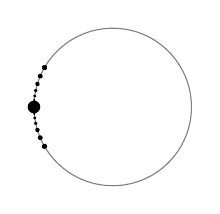
\begin{tikzpicture}
      \draw [gray] circle [radius=1];
      \fill (-1, 0) circle [radius=0.08];
      \foreach \rot in {3, 5, 8, 12, 17, 23, 30} {
        \pgfmathsetmacro\scal{0.01 * ln(\rot)};
        \fill [rotate=\rot] (-1, 0) circle [radius=\scal];
        \fill [rotate=-\rot] (-1, 0) circle [radius=\scal];
      }
    \end{tikzpicture}
  \end{center}
  Here orthogonality forces the eigenvalues to lie on the unit circle, and the fact that $I + T$ is compact means $-1$ is the only point in the essential spectrum.

  Thus, given any angle $\theta$, we can apply a spectral deformation to shrink all the points that are at most $\theta$ away from $-1$ to $-1$, and what is left is something in $\Omega_{k - 1}(n)$ for some $n$, since there are only finitely many eigenvalues at an angle $> \theta$ away from $-1$. By picking a spectral deformation that maps the unit circle to the unit circle and invariant under complex conjugation, this ensures the operator stays orthogonal and real. If we further choose it so that it is odd, then this preserves the set of operators that commute and anti-commute with it. So we stay inside $\Omega_{k - 1}$.

  In fact, given any compact subset of $\Omega_{k - 1}$, applying such a spectral deformation will send it to something lying in $\Omega_{k - 1}(n)$ for some large $n$. Thus, given any $a \in \Omega_{k - 1}(m)$, we can pick $\theta$ so that all the eigenvalues of $T$ are either $-1$ or $>\theta$ away from $-1$. Then the associated spectral deformation fixes $a$, but retracts any compact subset (and in particular, any image of maps from spheres) into one of the $\Omega_{k - 1}(n)$.

  In the case of $F_k^*(m)$, the spectrum instead looks like
  \begin{center}
    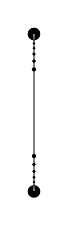
\begin{tikzpicture}
      \fill (0, 1) circle [radius=0.08];
      \fill (0, -1) circle [radius=0.08];
      \draw [gray] (0, 1) -- (0, -1);
      \foreach \rot in {3, 5, 8, 12, 17, 23, 30} {
        \pgfmathsetmacro\scal{0.008 * ln(\rot)};
        \pgfmathsetmacro\y{1 - 0.015 * \rot};
        \fill (0, \y) circle [radius=\scal];
        \fill (0, -\y) circle [radius=\scal];
      }
    \end{tikzpicture}
  \end{center}
  \qedshift
\end{proof}

Now it suffices to show that $\exp \pi: F^k_*(m) \to \Omega_{k - 1}(m)$ is a homotopy equivalence for all $m$. For convenience, set $H^k(m) = F^k_*(m) \setminus F^k_*(m - 1)$ and $D^k(m) = \Omega_{k - 1}(m) \setminus \Omega_{k - 1}(m - 1)$. We shall show that $\exp \pi: H^k(m) \to D^k(m)$ is a fiber bundle with contractible fiber for all $m$, and then use the following standard result in homotopy theory:
\begin{lemma}
  Let $(Y, Y_1, Y_2)$ and $(Z, Z_1, Z_2)$ be excisive triads, and $f: Y \to Z$ a map of triads. If
  \[
    f|_{Y_1}: Y_1 \to Z_1,\quad f|_{Y_2}: Y_2 \to Z_2,\quad f|_{Y_1 \cap Y_2} \to Z_1 \cap Z_2
  \]
  are all weak homotopy equivalences, then so is $f$.\fakeqed
\end{lemma}

We shall take
\begin{align*}
  Y &= F^k_*(m) & Y_1 &= F^k_*(m - 1)\\
  Z &= \Omega_{k - 1}(m) & Z_1 &= \Omega_{k - 1}(m - 1).
\end{align*}
By a simple spectral deformation argument, we can show that $F^k_*(n - 1)$ is the deformation retract of some open neighbourhood of $F_*^k(n)$ (add to $F_*^k(n - 1)$ those operators whose eigenvalue closest to $-1$ has small real part, then retract those to $-1$), and similarly for $\Omega_{k - 1}(n - 1)$ in a compatible way. We can then $Y_2$ and $Z_2$ to be these neighbourhoods.

By induction, we can conclude that $f|_{Y_1}$ is a homotopy equivalence. Then the fact that $\exp \pi$ restricts to a fiber bundle with contractible fiber shows that the other two maps are homotopy equivalences. 

\begin{thm}
  $\exp \pi: H^k(m) \to D^k(m)$ is a fiber bundle with contractible fiber.
\end{thm}

\begin{proof}
  Visually, the exponential map does something like this:
  \begin{center}
    \begin{tikzpicture}
      \fill [blue!30!red] (0, 1) circle [radius=0.08];
      \fill [blue!30!red] (0, -1) circle [radius=0.08];
      \draw [gray] (0, 1) -- (0, -1);
      \foreach \rot in {12, 17, 23, 30} {
        \pgfmathsetmacro\scal{0.01 * ln(\rot)};
        \pgfmathsetmacro\y{1 - 0.015 * \rot};
        \pgfmathsetmacro\col{\rot*2};

        \fill [blue!\col!red] (0, \y) circle [radius=\scal];
        \fill [blue!\col!red] (0, -\y) circle [radius=\scal];
      }

      \draw [->] (1, 0) -- (3, 0);
      \begin{scope}[shift={(5, 0)}]
        \draw [gray] circle [radius=1];
        \fill [blue!30!red] (-1, 0) circle [radius=0.08];
        \foreach \rot in {12, 17, 23, 30} {
          \pgfmathsetmacro\col{\rot*2};
          \pgfmathsetmacro\scal{0.01 * ln(\rot)};
          \fill [blue!\col!red, rotate=\rot] (-1, 0) circle [radius=\scal];
          \fill [blue!\col!red, rotate=-\rot] (-1, 0) circle [radius=\scal];
        }
      \end{scope}
    \end{tikzpicture}
  \end{center}
  Essentially, the ``information lost'' by passing from $T \in H^k(m)$ to $\exp \pi T \in D^k(m)$ is how the spectrum is distributed between $\pm i$.

  To make this concrete, observe that since $A \in D(n)$ is such that $I + A$ has constant rank $n$, it follows that $\ker (I + A)$ is a Hilbert space subbundle $\mathcal{H}$ of $D(n) \times H$ with orthogonal complement $\mathcal{H}^\perp$ an $n$-dimensional vector bundle.

  Given $T \in H^k(m)$, it acts on $\mathcal{H}$ and $\mathcal{H}^\perp$ disjointly. Its action on $\mathcal{H}^\perp$ is completely determined by $\exp \pi T$ (by linear algebra), and the action of $T$ on $\mathcal{H}$ is orthogonal, skew-Hermitian, etc. Thus, local triviality of $\mathcal{H}$ and $\mathcal{H}^\perp$ implies $\exp \pi: H^k(m) \to D^k(m)$ is a fiber bundle whose fiber consists of operators $T: H' \to H'$ (where $H'$ is any fiber of $\mathcal{H}$) that are
  \begin{enumerate}
    \item Orthogonal and square $-1$;
    \item Commuting with $J_1, \ldots, J_{k - 2}$ and anti-commuting with $J_{k - 1}$;
    \item If $k \equiv -1 \pmod 4$, then $J_1 \cdots J_{k - 2} T$ is not essentially definite.
  \end{enumerate}
  Equivalently, if we replace $B$ by $BJ_{k - 1}$ (thus reversing the previous shift), this is the number of choices of $J_k$ such that each irrep appears with infinite multiplicity. Thus, this is given by the quotient of the space of unitary $C_{k - 1}$-automorphisms of $H'$ by the centralizer of $J_k$, i.e.\ by the space of $C_k$-automorphisms of $H'$. Both of these are contractible. So we are done.
\end{proof}

\newpage
\section{Coda: The ABS Orientation}
Suppose $\pi: V \to X$ is a rank $k$ vector bundle with a Euclidean metric. Then taking the Clifford algebra with respect to (the negation of) the metric fiberwise gives us a $C_k$-bundle $C(V)$ over $X$. Let $M(V)$ be the Grothendieck group of $C(V)$-modules. If $E = E^0 \oplus E^1$ is a graded $C(V)$-module, then the pullbacks $\pi^* E_1$ and $\pi^* E_0$ are isomorphic over $V^\#$, the complement of the zero section, where the isomorphism at $v \in V^\#$ is given by multiplication by $v$ (with inverse a multiple of $v$, since $v^2 = -\|v\|$). This thus gives us an element of $\widetilde{KO}(V, V^\#) \cong \widetilde{KO}(X^V)$, where $X^V$ is the Thom space. In other words, we have a canonical map
\[
  M(V) \to \widetilde{KO}(X^V).
\]
Suppose $E$ came from a $C(V \oplus 1)$-module, then by a linear deformation, we can use a vector in the trivial factor as the isomorphism between $\pi^*E_1$ and $\pi^*E_2$ instead, and this extends to an isomorphism defined on all of $V$. So the resulting class is trivial in $\widetilde{KO}(X^V)$. Moreover, this map is natural with respect to products, namely if $V \to X$ and $W \to Y$ are two bundles, then the following diagram commutes:
\begin{useimager}
  \[
    \begin{tikzcd}
      A(V) \otimes A(W) \ar[d] \ar[r] & A (V \oplus W) \ar[d]\\
      \widetilde{KO}(X^V) \otimes \widetilde{KO}(Y^W) \ar[r] & \widetilde{KO}(X \times Y^{V \oplus W}).
    \end{tikzcd}
  \]
\end{useimager}
In particular, taking $X = *$, we obtain \emph{ring} homomorphisms
\[
  A_* \to \sum_{k \geq 0} KO^{-k}(*)
\]
In fact, this is the same map as the one we constructed above, which is just a matter of tracing through all the constructions we have done.

Let $\GSpin(k)$ be the even invertible elements of $C_k$ that preserve $\R^k \subseteq C_k$ under the conjugation action, and let $\Spin(k)$ consist of those elements of ``spinor norm'' $1$. The natural action on $\R^k$ begets a map $\Spin(k) \to \SO(k)$ that is a non-trivial double cover. Crucially, $\Spin(k)$ acts as automorphisms of the whole of $C_k$.

Thus, $V$ has the structure of a $\Spin(k)$-bundle, so that there is a principal $\Spin(k)$-bundle $P \to X$ with $V = P \times_{\Spin(k)} \R^k$, then $C(V) = P \times_{\Spin(k)} C_k$ and there is a natural map $A_k \to A(V)$ that sends an $C_k$ module $M$ to $P \times_{\Spin(k)} M$. This gives a long composite
\[
  A_k \to \widetilde{KO}(X^V).
\]
In particular, if $k = 8m$, and $\lambda$ is the generator of $A_{8m}$, then by naturality, the image of $\lambda^m$ restricts to a generator of $\widetilde{KO}(S^{8m})$. So this is a Thom class of the bundle $V$. Stabilizing, we get

\begin{thm}
  Every spin bundle is naturally $KO$-oriented.
\end{thm}

\bibliographystyle{plain}
\bibliography{clifford}

\end{document}
